%!TEX TS-program = xelatex
%!TEX encoding = UTF-8 Unicode
%!TEX root = ../kabala.tex
\begin{tikzpicture}
  \draw (-8.5,-8.5) rectangle (29.3,12.5);

  \node[align=left, anchor=west, font=\fontsize{42}{42}] at (-7.5,10) {\emph{Autocostruzione di un interprete.} \\ \emph{Per quale Musica?}};
  \node[anchor=north west, inner sep=0pt] (mari) at (11,8) {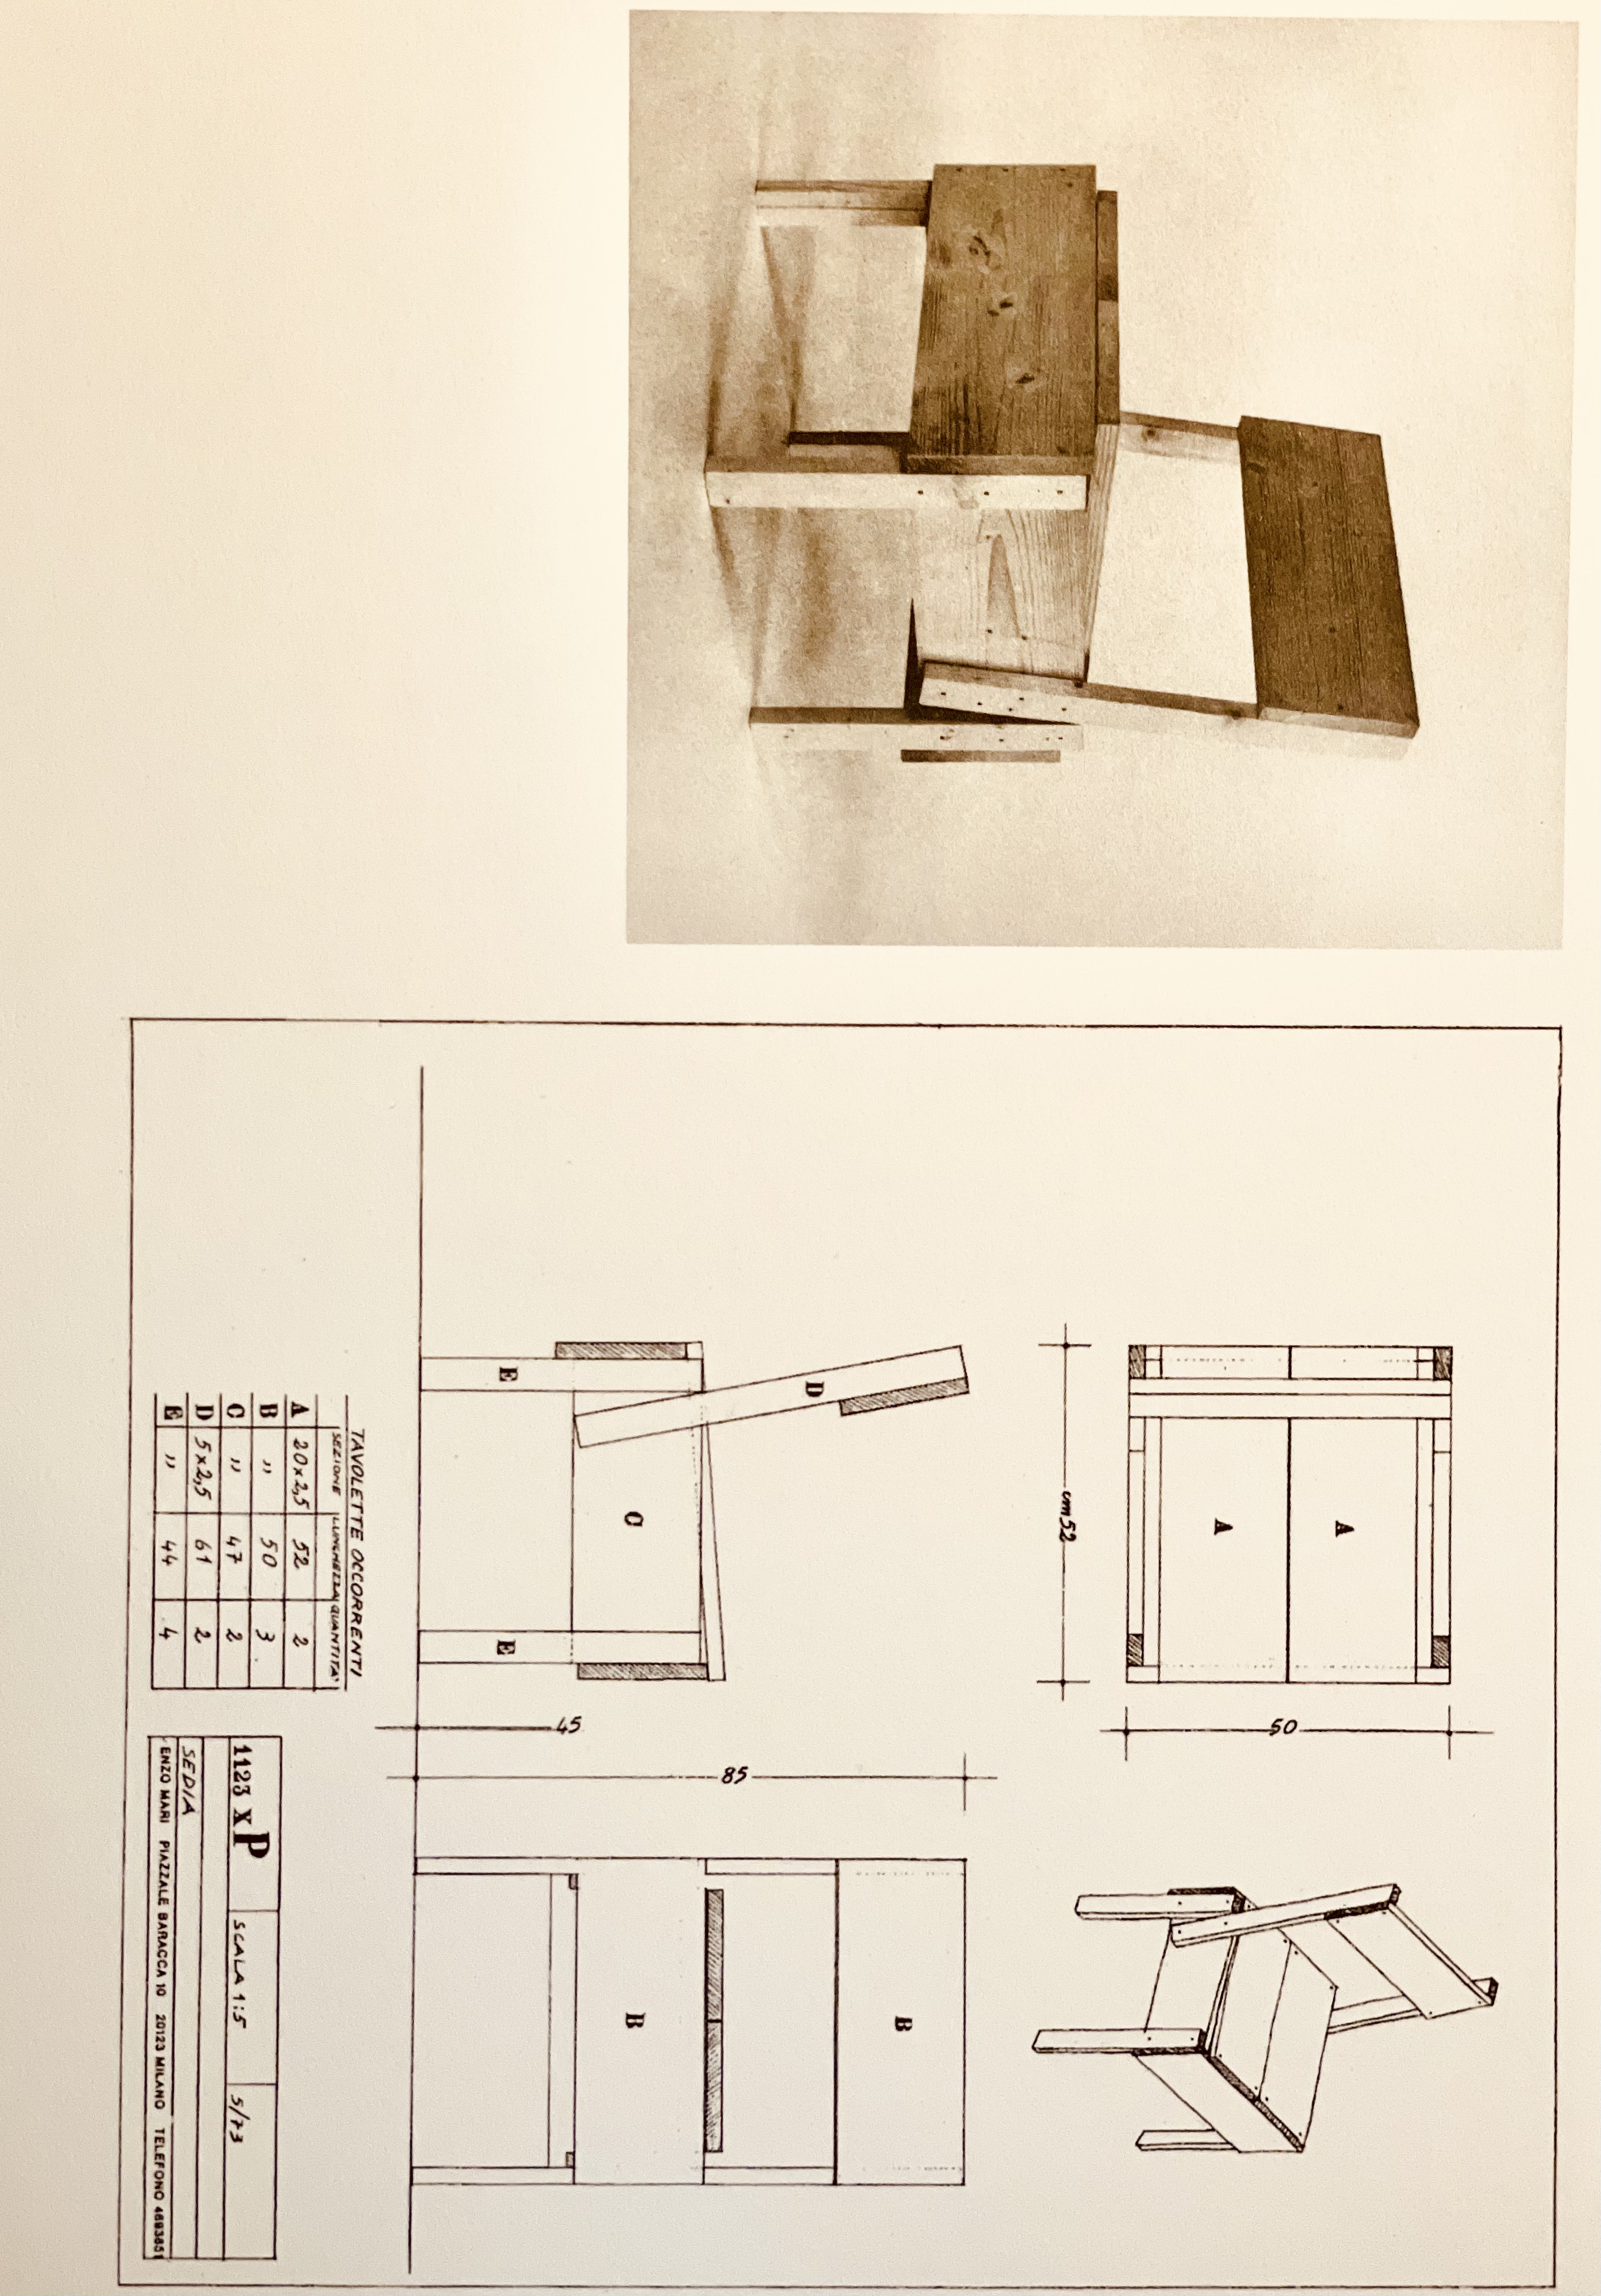
\includegraphics[width=15cm]{images/1-mari-b.jpg}};
  \node[align=left, anchor=west, font=\fontsize{23}{23}] at (11,-4) {\emph{testo}};

  \def\r{2.5}
  % centro
  \draw (0,0) circle (\r) coordinate (sei);
  % esagono
  \draw [very thin, name path=a30] (30:\r) circle (\r) coordinate (quattro);
  \draw [very thin, name path=a90] (90:\r) circle (\r);
  \draw [very thin, name path=a150] (150:\r) circle (\r) coordinate (cinque);
  \draw [very thin, name path=a210] (210:\r) circle (\r) coordinate (sette);
  \draw [very thin, name path=a270] (270:\r) circle (\r) coordinate (nove);
  \draw [very thin, name path=a330] (330:\r) circle (\r) coordinate (otto);
  % periferia
  %\draw (0:\r*2) circle (\r);
  \draw [very thin, name path=b30] (30:\r*2) circle (\r);
  % \draw (60:\r*2) circle (\r);
  \draw [very thin, name path=b90] (90:\r*2) circle (\r) coordinate (uno);
  % \draw (120:\r*2) circle (\r);
  \draw [very thin, name path=b150] (150:\r*2) circle (\r);
  % \draw (180:\r*2) circle (\r);
  \draw [very thin, name path=b210] (210:\r*2) circle (\r);
  % \draw (240:\r*2) circle (\r);
  \draw [very thin, name path=b270] (270:\r*2) circle (\r) coordinate (dieci);
  % \draw (300:\r*2) circle (\r);
  \draw [very thin, name path=b330] (330:\r*2) circle (\r);
  % bordo
  %\draw[red] (0,0) circle (\r*2);
  \draw[very thick] (0,0) circle (\r*3);
  \draw[very thick] (0,0) circle (\r*3.1);

  \path [name intersections={of=a30 and b30,by=b60}];
  \path [name intersections={of=a150 and b150,by=b120}];
  \path [name intersections={of=a210 and b210,by=b180}];
  \path [name intersections={of=a270 and b270,by=b240}];
  \path [name intersections={of=a330 and b270,by=b300}];
  \path [name intersections={of=a330 and b330,by=b360}];

  % \fill [] (b60) circle (2pt);
  % \fill [] (b120) circle (2pt);
  % \fill [] (b180) circle (2pt);
  % \fill [] (b240) circle (2pt);
  % \fill [] (b300) circle (2pt);
  % \fill [] (b360) circle (2pt);
  \draw [very thin, name path=b60] (b60) circle (\r);
  \draw [very thin, name path=b120] (b120) circle (\r);
  \draw [very thin, name path=b180] (b180) circle (\r);
  \draw [very thin, name path=b240] (b240) circle (\r);
  \draw [very thin, name path=b300] (b300) circle (\r);
  \draw [very thin, name path=b360] (b360) circle (\r);

  \draw [very thin] (30:\r*3) arc (90:270:\r) arc (90:210:\r);
  \draw [very thin] (30:\r*3) arc (-30:-210:\r) arc (-30:-150:\r);
  \draw [very thin] (90:\r*3) arc (30:-150:\r) arc (30:-90:\r);
  \draw [very thin] (90:\r*3) arc (-210:-30:\r);
  \draw [very thin] (150:\r*3) arc (-150:30:\r);
  \draw [very thin] (150:\r*3) arc (90:-90:\r);
  \draw [very thin] (210:\r*3) arc (150:-30:\r);
  \draw [very thin] (210:\r*3) arc (-90:90:\r);
  \draw [very thin] (270:\r*3) arc (-30:150:\r) arc (-30:90:\r);
  \draw [very thin] (270:\r*3) arc (210:30:\r);
  \draw [very thin] (330:\r*3) arc (270:90:\r) arc (270:150:\r);
  \draw [very thin] (330:\r*3) arc (30:210:\r) arc (30:150:\r);

  \draw [very thin] (90:\r*3) arc (330:270:\r) arc (330:270:\r) arc (330:270:\r)
                  arc (30:-30:\r)  arc (30:-30:\r)  arc (30:-30:\r)
                  arc (90:30:\r)   arc (90:30:\r)   arc (90:30:\r)
                  arc (150:90:\r)  arc (150:90:\r)  arc (150:90:\r)
                  arc (210:150:\r) arc (210:150:\r) arc (210:150:\r)
                  arc (270:210:\r) arc (270:210:\r) arc (270:210:\r);


  \draw[ultra thick, accent] (uno) -- (b60) -- (quattro) -- (sei) -- (cinque) -- (b120) -- (uno) -- (dieci);
  \draw[ultra thick, accent] (cinque) -- (quattro) -- (otto) -- (nove) -- (sette) -- (cinque);
  \draw[ultra thick, accent] (sette) -- (dieci) -- (otto);
  \draw[ultra thick, accent] (sette) -- (sei) -- (otto) -- (sette);
  \draw[ultra thick, accent] (b60) -- (sei) -- (b120) -- (b60);

  \tikzset{dot/.style = {draw=accent, ultra thick, double=LeaPurple, circle, fill=LeaPurple, minimum size=2cm,inner sep=0pt, outer sep=0pt}}

  \node [dot] (nsei) at (sei) {\hyperlink{page.6}{\small LUZ}};
  \node [dot] (nquattro) at (quattro) {\hyperlink{page.4}{\small STRUMENTO}};
  \node [dot] (ndue) at (b60) {\hyperlink{page.3}{\small INTERPRETE}};
  \node [dot] (nuno) at (uno) {\hyperlink{page.1}{\small MARI}};
  \node [dot] (ntre) at (b120) {\hyperlink{page.2}{\small RACCONTO}};
  \node [dot] (ncinque) at (150:\r) {\hyperlink{page.5}{\small S-R-T-S}};
  \node [dot] (nsette) at (210:\r) {\hyperlink{page.7}{\small COME?}};
  \node [dot] (nnove) at (270:\r) {\hyperlink{page.9}{\small LAZZARO}};
  \node [dot] (ndieci) at (270:\r*2) {\hyperlink{page.10}{\small DIDATTICA}};
  \node [dot] (notto) at (330:\r) {\hyperlink{page.8}{\small COME\ldots}};
\end{tikzpicture}
